\documentclass{article}

\usepackage{amsmath,amssymb,amsthm}

\begin{document}
 
\section*{Problem 1}
 A football team of 11 players is to be selected from a set of 15 players, 5 of whom can play only in the backfield, 8 of whom can play only on the line, and 2 of whom can play either in the backfield or on the line. Assuming a football team has 7 men on the line and 4 men in the backfield, determine the number of football teams possible.
    
 	\subsection*{Solution}
     \\
     Let ${O} = |O| = 8$ be the number of available online players. \\
     Let ${B} = |B| = 5$ be the number of available backfield players. \\
     Let ${A} = |A| = 2$ be the number of available adaptable players. \\
     \\
     Also, \\
 	Let ${T} = |T| = 11$ be the team to be chosen. \\
     Let ${O'} = |O'| = 7$ be the number of online players to be chosen. \\
     Let ${B'} = |B'| = 4$ be the number of backfield players to be chosen. \\
     \\
     Then we can define the following cases: 
     \\ \\
     \textbf{Case 1: ${A}$ is not in ${T}$.}
     \\
     If ${T}$ contains no players from ${A}$ then we can only choose from ${B}$ and ${O}$. \\ 
     This gives us: \\
     $$\binom{8}{7} \binom{5}{4} = (8)(5) = 40$$
     \\ \\
     \textbf{Case 2: Exactly one player from ${A}$ is in ${T}$.}
     \\ \\
     If exactly one player from ${A}$ is chosen for ${T}$ then either $a_{1} \in {O}$ or $a_{1} \in {B}$. \\
     \begin{itemize}
         \item If $a_{1} \in {O}$ then we have: \\
     $$(2) \binom{8}{6} \binom{5}{4} = \frac{8!}{6!(8-6)!} \times \frac{5!}{4!(5-4)!} = (2) \frac{54321}{4321(1)} \frac{87654321}{654321(21)} = (10)(28) = 280$$
     \\ \\
         \item If $a_{1} \in {B}$ then we have: \\
      $$\binom{8}{7} (2) \binom{5}{3} = \frac{8!}{7!(8-7)!} \times \frac{5!}{3!(5-3)!} = \frac{87654321}{654321(1)} (2) \frac{54321}{321(21)} = (8)(20) = 160$$
     \end{itemize}
     \\ \\ 
     So if $a_{1}$ is either in ${A}$ or in ${B}$ then we have $160+280 = 440$ ways to arrange the available team members into a team. 
     \\ \\
     \textbf{Case 3: Both members of ${A}$ are in ${T}$.} 
     \\ \\
     \begin{itemize}
         \item Either both $a_{1}$ and $a_{2}$ are in ${B}$.
         \item Both $a_{1}$ and $a_{2}$ are in ${O}$.
         \item Either $a_{1} \in {B}$ and $a_{2} \in {O}$, or it is the other way around. It makes no difference. 
     \end{itemize}
     \\ \\
     \begin{itemize}
         \item If both $a_{1}$ and $a_{2}$ are in ${B}$ then we have: \\
         $$\binom{8}{7} \binom{5}{2} = \frac{8!}{7!(8-7)!} \times \frac{5!}{2!(5-2)!} = (8)(10) = 80.$$
         \item If both  $a_{1}$ and $a_{2}$ are in ${O}$ then we have: \\
         $$\binom{8}{5} \binom{5}{4} = \frac{8!}{5!(8-5)!} \times \frac{5!}{4!(5-4)!} = (56)(5) = 280.$$
         \item If $a_{1} \in {B}$ and $a_{2} \in {O}$ (or vice-versa) we have: \\
         $$\binom{5}{3} \binom{8}{5} = \frac{5!}{3!(5-3)!} \times \frac{5!}{3!(5-3)!} \frac{8!}{6!(8-6)!} = (56)(5) = 280.$$
         \item but there are two ways this last placement can be arranged so $2(280) = 560$. 
     \end{itemize}
     Finally the total number of ways to arrange all available players into a team of 11 players is the sum: \\
     $$40 + 440 + 80 + 280 + 280 + 560 = 1680$$
     
\pagebreak

\section*{Problem 2}
A classroom has two rows of eight seats each. There are 14 students, 5 of whom always sit in the front row and 4 of whom always sit in the back row. In how many ways  can the students be seated?

\subsection*{Solution}
    \begin{itemize}
        \item 5 ALWAYS sit in front $\binom{8}{5}$
        \item 4 ALWAYS sit in the back $\binom{8}{4}$
        \item 5 students left sit wherever they feel like it in $(16-9) = 7$ seats. So there are $\binom{7}{5}$ for those remaining students. 
        \item so we have that $56 \times 70 \times 21 = 82320$ ways they could sit.
    \end{itemize}
    
\section*{Problem 3}
 We are given eight rooks, five of which are red and three of which are blue.
 \begin{itemize}
     \item In how many ways can the eight rooks be placed on an 8-by-8 chessboard so that no two rooks can attack one another?
     \item \textbf{Solution: }
     \item Choose the three blue rooks there are $\binom{8}{3}$ rows to place them. Once they are placed there are $8 \times 7$ choices for the chosen rows. So there are $\binom{8}{3} \times 8 \times 7 \times 6$ ways to place the two blue rooks. 
     \item For the remaining 5 red rooks there is a placement with respect to the chosen place of each of the blue already placed. There are 5 rows remaining and 5 rooks so we have $\binom{5}{5}$ ways to place the rooks. 
     \item To place them in each column there are 5 columns for the 3 rows this is $5 \times 4 \times 3 \times 2$ ways to choose these rows.
     \item So there are $\binom{6}{4} \times 6 \times 5 \times 4 \times 3 \times 2$ ways to place the 5 red rooks on the board.
     \item So we have $$(\frac{(8 \times 7 \times 6)^{2}}{3!})(\frac{(5 \times 4 \times 3 \times 2)^{2}}{5!})$$ \\ 
 ways to place the rooks where they cant attack three other rooks.
 \end{itemize}
 
\section*{Problem 4}
 How many permutations are there of the letters of the word 'ADDRESSES'?
         \begin{itemize}
             \item There is 1 A, 2 D's, 1 R, 2 E's, and 3 S's.
             \item There are 9 total letters
             \item To make up for all that over counting we have: $$\frac{9!}{3!3!2!2!1!1!} = 2520$$
         \end{itemize}
         
\section*{Problem 5}
A secretary works in a building located nine blocks east and eight block north of his home.
Every day he walks 17 blocks to work. (See the map that follows.)
\begin{itemize}
    \item How many different routes are possible for him?
    \item How many different routes are possible if the one block in the easterly direction, which begins four block east and three blocks north of his home,
is under water (and he can't swim)? (Hint: use subtraction principle)
\end{itemize}
\\ \\
\begin{center}
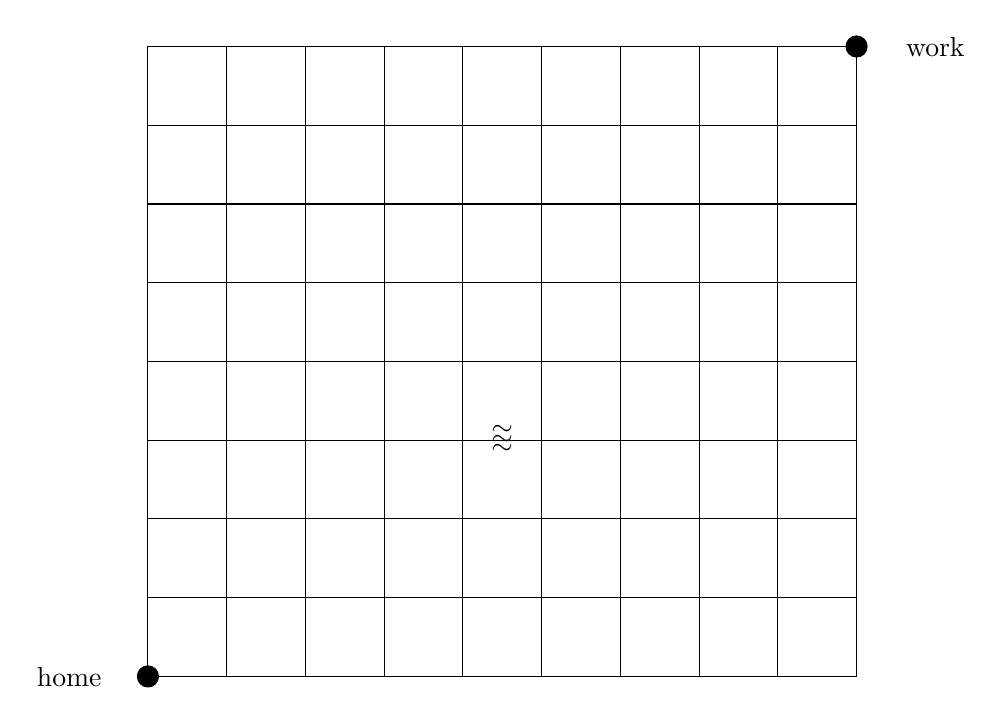
\begin{tikzpicture}
\draw
\foreach \x in {0,1,...,8} { (0,\x) -- (9,\x) (\x,0) -- (\x,8)}
(9,0) -- (9,8)
(-1,0) node {home} (10,8) node {work}
(4.5,3) node {$\sim$} (4.5,3.12) node {$\sim$} (4.5,2.88) node {$\sim$};
\fill (0,0) circle (4pt) (9,8) circle (4pt) ;
\end{tikzpicture}
\end{center}
\\ \\
\textbf{Solution: }
\\
He walks 17 blocks in all so x blocks in one direction or y blocks in the other with south and west unavailable. So the total blocks is $x + y = 17$ and so we can pick $\binom{17}{x}$ or $\binom{17}{y}$ but they are equal. So we have that $\mathcal{P}(x+y, x, y) = \mathcal{P}(17, x, y) = \mathcal{P}(17, 8, 9) = \mathcal{P}(17, 9, 8) = \frac{17!}{8!9!} = 24310.$

\end{document}
